\documentclass[hyperref, a4paper]{article}

\usepackage{geometry}
\usepackage{titling}
\usepackage{titlesec}
% No longer needed, since we will use enumitem package
% \usepackage{paralist}
\usepackage{enumitem}
\usepackage{footnote}
\usepackage{amsmath, amssymb, amsthm}
\usepackage{mathtools}
\usepackage{bbm}
\usepackage{cite}
\usepackage{graphicx}
\usepackage{subcaption}
\usepackage{physics}
\usepackage{tensor}
\usepackage{siunitx}
\usepackage[version=4]{mhchem}
\usepackage{tikz}
\usepackage{xcolor}
\usepackage{listings}
\usepackage{underscore}
\usepackage{autobreak}
\usepackage[ruled, vlined, linesnumbered]{algorithm2e}
\usepackage{nameref,zref-xr}
\zxrsetup{toltxlabel}
\usepackage[colorlinks,unicode]{hyperref} % , linkcolor=black, anchorcolor=black, citecolor=black, urlcolor=black, filecolor=black
\usepackage[most]{tcolorbox}
\usepackage{prettyref}

% Page style
\geometry{left=3.18cm,right=3.18cm,top=2.54cm,bottom=2.54cm}
\titlespacing{\paragraph}{0pt}{1pt}{10pt}[20pt]
\setlength{\droptitle}{-5em}

% More compact lists 
\setlist[itemize]{
    %itemindent=17pt, 
    %leftmargin=1pt,
    listparindent=\parindent,
    parsep=0pt,
}

\setlist[enumerate]{
    %itemindent=17pt, 
    %leftmargin=1pt,
    listparindent=\parindent,
    parsep=0pt,
}

% Math operators
\DeclareMathOperator{\timeorder}{\mathcal{T}}
\DeclareMathOperator{\diag}{diag}
\DeclareMathOperator{\legpoly}{P}
\DeclareMathOperator{\primevalue}{P}
\DeclareMathOperator{\sgn}{sgn}
\DeclareMathOperator{\res}{Res}
\newcommand*{\ii}{\mathrm{i}}
\newcommand*{\ee}{\mathrm{e}}
\newcommand*{\const}{\mathrm{const}}
\newcommand*{\suchthat}{\quad \text{s.t.} \quad}
\newcommand*{\argmin}{\arg\min}
\newcommand*{\argmax}{\arg\max}
\newcommand*{\normalorder}[1]{: #1 :}
\newcommand*{\pair}[1]{\langle #1 \rangle}
\newcommand*{\fd}[1]{\mathcal{D} #1}
\DeclareMathOperator{\bigO}{\mathcal{O}}

% TikZ setting
\usetikzlibrary{arrows,shapes,positioning}
\usetikzlibrary{arrows.meta}
\usetikzlibrary{decorations.markings}
\usetikzlibrary{calc}
\tikzstyle arrowstyle=[scale=1]
\tikzstyle directed=[postaction={decorate,decoration={markings,
    mark=at position .5 with {\arrow[arrowstyle]{stealth}}}}]
\tikzstyle ray=[directed, thick]
\tikzstyle dot=[anchor=base,fill,circle,inner sep=1pt]

% Algorithm setting
% Julia-style code
\SetKwIF{If}{ElseIf}{Else}{if}{}{elseif}{else}{end}
\SetKwFor{For}{for}{}{end}
\SetKwFor{While}{while}{}{end}
\SetKwProg{Function}{function}{}{end}
\SetArgSty{textnormal}

\newcommand*{\concept}[1]{{\textbf{#1}}}

% Embedded codes
\lstset{basicstyle=\ttfamily,
  showstringspaces=false,
  commentstyle=\color{gray},
  keywordstyle=\color{blue}
}

\lstdefinestyle{console}{
    basicstyle=\footnotesize\ttfamily,
    breaklines=true,
    postbreak=\mbox{\textcolor{red}{$\hookrightarrow$}\space}
}

% Reference formatting
\newrefformat{fig}{Figure~\ref{#1}}

% Color boxes
\tcbuselibrary{skins, breakable, theorems}
\newtcbtheorem[number within=section]{warning}{Warning}%
  {colback=orange!5,colframe=orange!65,fonttitle=\bfseries, breakable}{warn}
\newtcbtheorem[number within=section]{note}{Note}%
  {colback=green!5,colframe=green!65,fonttitle=\bfseries, breakable}{note}
\newtcbtheorem[number within=section]{info}{Info}%
  {colback=blue!5,colframe=blue!65,fonttitle=\bfseries, breakable}{info}

% Displaying texts in bookmarkers

\pdfstringdefDisableCommands{%
  \def\\{}%
  \def\ce#1{<#1>}%
}

\pdfstringdefDisableCommands{%
  \def\texttt#1{<#1>}%
  \def\mathbb#1{#1}%
}
\pdfstringdefDisableCommands{\def\eqref#1{(\ref{#1})}}

\makeatletter
\pdfstringdefDisableCommands{\let\HyPsd@CatcodeWarning\@gobble}
\makeatother

\newenvironment{shelldisplay}{\begin{lstlisting}}{\end{lstlisting}}

\newcommand{\shortcode}[1]{\texttt{#1}}

\lstset{style = console}

% Make subsubsection labeled
\setcounter{secnumdepth}{4}
\setcounter{tocdepth}{4}

\newcommand*{\laplace}{\mathcal{L}}
\newcommand*{\fourier}{\mathcal{F}}
\newcommand*{\zerotoinf}{\int_{0}^{\infty}}
\newcommand*{\inftoinf}{\int_{-\infty}^{\infty}}

\title{Homework 3}
\author{Jinyuan Wu}

\begin{document}

\maketitle

\section{}

By convolution theorem we have 
\begin{equation}
    \begin{aligned}
        \fourier^{-1}\left[
            \frac{1}{(1 + \ii \omega) (2 + \ii \omega)}
        \right] &= 
        \fourier^{-1} \left[
            \frac{1}{1 + \ii \omega}
        \right] \otimes
        \fourier^{-1} \left[
            \frac{1}{2 + \ii \omega}
        \right]
        = \ee^{-x} H(x) \otimes \ee^{-2x} H(x) \\
        &= \inftoinf \ee^{- x'} H(x') \ee^{-2 (x - x')} H(x - x') \dd{x'} \\
        &= \ee^{- 2x} \int_{0}^{x} H(x) \ee^{x'} \dd{x'} = 
        (\ee^{-x} - \ee^{-2x}) H(x).
    \end{aligned}
\end{equation}

\section{}\label{sec:prob-2}

We need to solve 
\begin{equation}
    \begin{gathered}
        u_t=4 u_{x x} \text { for } 0<x<L, t>0 \\
        u(0, t)=u(L, t)=0, \\
        u(x, 0)=x^2(L-x).
    \end{gathered}
\end{equation}
This can be done by standard separation of variables.
Suppose $u = X T$.
We have 
\[
    X T' = 4 T X'' \Rightarrow \frac{X''}{X} = \frac{T'}{4T} = \lambda.
\]
Since the boundary conditions require that 
\[
    X(0) = X(L) = 0,
\]
$X$ can't be exponential, and we have $\lambda = - k^2$,
and the $x$ part of the problem is then 
\[
    X'' + k^2 X = 0, \quad X(0) = X(L) = 0.
\]
This just gives us an odd Fourier series: 
we have 
\[
    X = A \cos (kx) + B \sin (kx),
\]
and since $X(0) = 0$, $A = 0$, 
and since $X(L) = 0$, we have 
\[
    k L = \pi n, \quad n \in \mathbb{Z}.
\]
The set of independent $X$s is therefore 
\begin{equation}
    X_n = \sin(k_n x), \quad k_n = \frac{\pi n }{L}, \quad n = 1, 2, \ldots
\end{equation}
The $t$ part of the problem is then 
\[
    T'_n + 4 k_n^2 T_n = 0,
\]
\begin{equation}
    T_n = T_n(0) \ee^{- 4 k_n^2 t}.
\end{equation}
The general solution is therefore 
\begin{equation}
    u = \sum_{n =1}^\infty c_n \sin(k_n x) \ee^{- 4 k_n^2 t}, \quad k_n = \frac{\pi n}{L}.
\end{equation}
Now we apply the initial condition.
We have 
\[
    \sum_{n =1}^\infty c_n \sin(\frac{\pi n}{L} x) = x^2(L-x),
\]
and therefore 
\begin{equation}
    \frac{L}{2} \cdot c_n = \int_{0}^{L} \sin(\frac{\pi n}{L} x) x^2(L-x) \dd{x}
    = - \frac{L^4}{(n \pi)^4} (2 \pi n + 4 \pi n (-1)^n),
\end{equation}
and 
\begin{equation}
    u(x, t) = - \sum_{n=1}^{\infty} \frac{4 L^3 (1 + 2 (-1)^n)}{(n \pi)^3} \sin(\frac{\pi n}{L} x) \ee^{- 4 (\pi n / L)^2 t}.
\end{equation}

\section{}

Since 
\[
    (a \cos \omega x + b \sin \omega x) \ee^{- \omega^2 k t} 
\]
is a specific solution of 
\begin{equation}
    \pdv{u}{t} = k \pdv[2]{u}{x},
\end{equation}
the general solution is 
\begin{equation}
    u(x, t) = \int_{0}^{\infty} (a_\omega \cos \omega x + b_\omega \sin \omega x) \ee^{- \omega^2 k t} \dd{\omega}.
\end{equation}
The initial condition 
\begin{equation}
    u(x, t=0) = f(x) = \begin{cases}
        \ee^{-x}, &\quad \abs{x} \leq 1, \\
        0, &\quad \abs{x} > 1
    \end{cases}
\end{equation}
means 
\[
    \int_{0}^{\infty} (a_\omega \cos \omega x + b_\omega \sin \omega x) \dd{\omega} = f(x),
\]
and since  
\begin{equation}
    \inftoinf \cos \omega x \cos \omega' x \dd{x} = \pi \delta(\omega + \omega') + \pi \delta(\omega - \omega'), \quad 
    \inftoinf \sin \omega x \sin \omega' x \dd{x} = \pi \delta(\omega - \omega') - \pi \delta (\omega + \omega'),
\end{equation}
we have 
\begin{equation}
    \pi a_\omega = \inftoinf f(x) \cos (\omega x) \dd{x}
    = \int_{-1}^{1} \ee^{-x} \cos (\omega x) \dd{x}
    = \frac{\left(1+\ee^2\right) \omega  \sin
    (\omega )+\left(\ee^2-1\right) \cos
    (\omega )}{\ee \left(\omega ^2+1\right)},
\end{equation}
\begin{equation}
    \pi b_\omega = \inftoinf f(x) \sin (\omega x) \dd{x}
    = \int_{-1}^{1} \ee^{-x} \sin (\omega x) \dd{x}
    = \frac{\left(\ee^2-1\right) \omega  \cos
    (\omega )-\left(1+\ee^2\right) \sin
    (\omega )}{\ee \left(\omega ^2+1\right)}.
\end{equation}
So we have 
\begin{equation}
    \begin{aligned}
        u(x, t) = \frac{1}{\pi} \int_{0}^{\infty} \ee^{- \omega^2 k t} 
        &\Bigg(
            \frac{\left(1+\ee^2\right) \omega  \sin
            (\omega )+\left(\ee^2-1\right) \cos
            (\omega )}{\ee \left(\omega ^2+1\right)}
            \cos (\omega x) \\
        &\quad + \frac{\left(\ee^2-1\right) \omega  \cos
            (\omega )-\left(1+\ee^2\right) \sin
            (\omega )}{\ee \left(\omega ^2+1\right)}
            \sin (\omega x)
        \Bigg)  \dd{\omega}.
    \end{aligned}
\end{equation}

We can also write the solution using the heat kernel 
\begin{equation}
    u(x, t) = \frac{1}{2 \sqrt{\pi k t}} \int_{-\infty}^{\infty} f(\xi) \ee^{-(x-\xi)^2 / 4 k t} \dd \xi
    = \frac{1}{2 \sqrt{\pi k t}} \int_{-1}^{1} \ee^{-x} \ee^{-(x-\xi)^2 / 4 k t} \dd{\xi} .
\end{equation}

\section{}

The problem is 
\begin{equation}
    \begin{gathered}
        y_{t t}=c^2 y_{x x} \text { for } 0<x<L, t>0 \\
        y(0, t)=y(L, t)=0, \\
        y(x, 0)=f(x), \\
        y_t(x, 0)=g(x)
        \end{gathered}
\end{equation}
Again we use separation of variables.
Suppose 
\[
    y = X T.
\]
We have 
\[
    X T'' = c^2 T X'' \Rightarrow 
    \frac{X''}{X} = \frac{T''}{c^2 T} = \lambda, 
\]
and again because the boundary conditions, we can only have $\lambda < 0$, 
and therefore $\lambda = - k^2$, and 
\begin{equation}
    X'' + k^2 X = 0, 
\end{equation}
and repeating the procedure in \prettyref{sec:prob-2},
we get 
\begin{equation}
    X_n = \sin k_n x , \quad k_n = \frac{n \pi}{L}.
\end{equation}
The corresponding solution for the $T$ equation is 
\begin{equation}
    T_n'' + k_n^2 c^2 T_n = 0 \Rightarrow 
    T_n = a_n \cos (k_n c t) + b_n \sin (k_n c t).
\end{equation}
The general solution is therefore 
\begin{equation}
    y(x, t) = \sum_{n=0}^{\infty} (a_n \cos (k_n c t) + b_n \sin (k_n c t)) \sin k_n x,
    \quad k_n = \frac{n \pi}{L}.
\end{equation}

Now we take 
\begin{equation}
    c = 5, \quad L = \pi, \quad f(x)=\sin 2 x, \quad g(x)=\pi-x.
\end{equation}
We have 
\[
    \sum_{n=0}^{\infty} a_n \sin n x = \sin 2 x,  
\]
and 
\begin{equation}
    a_2 = 1, \quad a_n = 0, \quad n \neq 2.
\end{equation}
The $g(x)$ condition means 
\[
    \sum_{n=0}^{\infty} b_n \cdot 5n \cdot \sin n x = \pi - x,
\]
\[
    \frac{L}{2} \cdot b_n \cdot n c = \int_{0}^{\pi} (\pi - x) \sin n x \dd{x}
    = \frac{\pi}{n} 
    \Rightarrow b_n = \frac{2 }{ 5 n^2}  .
\]
So we have 
\begin{equation}
    y(x, t) = \sum_{n=0}^{\infty} \frac{2}{5n^2} \sin (5 n t) \sin (n x) + \cos (5 n t) \sin (2 x). 
\end{equation}

\section{}

The wave function with velocity $c$ has the following general solution:
\begin{equation}
    y(x, t)=\frac{1}{2} f(x-c t)+\frac{1}{2} f(x+c t)+\frac{1}{2 c} \int_{x-c t}^{x+c t} g\left(x^{\prime}\right) \mathrm{d} x^{\prime} .
\end{equation}
When $c = 2$, $f(x) = 0$, and 
\begin{equation}
    g(x)=\left\{\begin{array}{rr} 
        & 1 \text { for } \quad 0 \leqslant x \leqslant 2 \\
        -1 & \text { for }-2 \leqslant x<0 \\
        & 0 \text { for } \quad|x|>2
        \end{array}\right.,
\end{equation}
we have 
\begin{equation}
    \begin{aligned}
        y(x, t) &= \frac{1}{4} \int_{\max(x - 2 t, -2)}^{\min (x + 2 t, 2)} g(x') \dd{x'} \\
        &= \frac{1}{4} \begin{cases}
            0 , &\quad \max(x-2t, -2) \geq 2, \\
            \min(x + 2t , 2) - \max(x - 2t, -2) , &\quad 0 < \max(x-2t, -2) < 2, \\
            \min(x + 2t , 2) + \max(x - 2t, -2), &\quad  \max(x-2t, -2) \leq 0 \leq \min(x + 2t , 2), \\
            -  \min(x + 2t , 2) + \max(x - 2t, -2), &\quad \min(x + 2t , 2) < 0, \\
            0, &\quad \min(x + 2t, 2) \leq -2.
        \end{cases} 
    \end{aligned}
\end{equation}
Plots of $y(x, t)$ are shown in \prettyref{fig:plot-y}.

\begin{figure}
    \centering
    \begin{subfigure}{0.3\textwidth}
        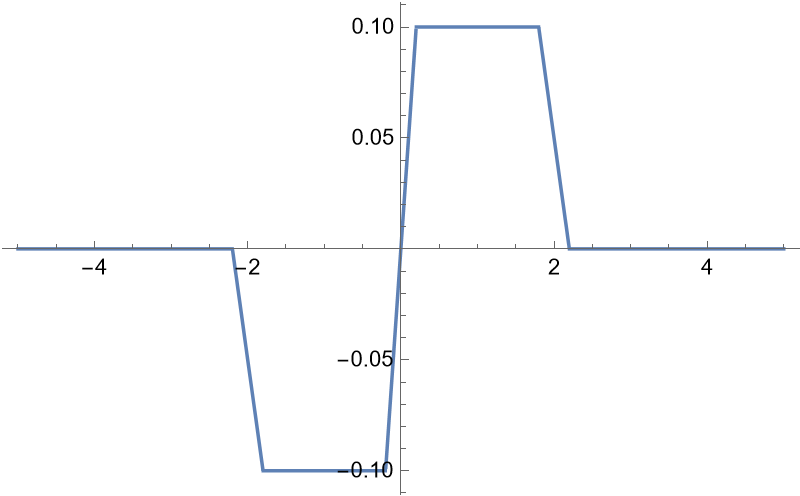
\includegraphics[width=\textwidth]{plots/config-0.1.png}
        \subcaption{$t=0.1$}
    \end{subfigure}
    \begin{subfigure}{0.3\textwidth}
        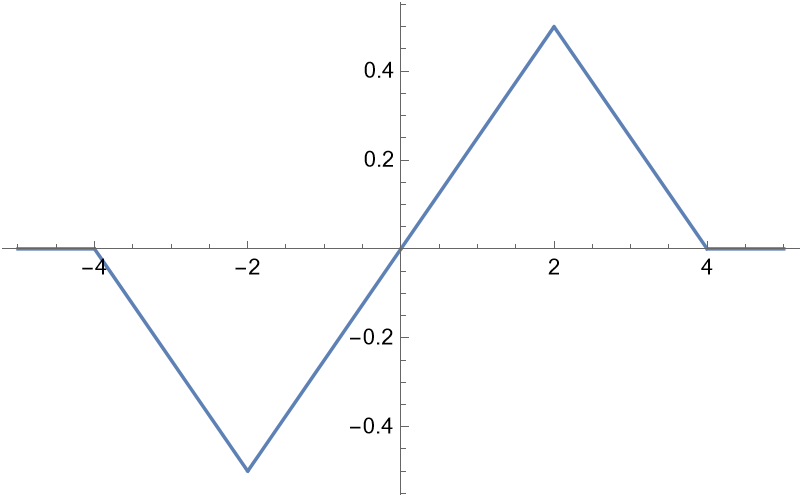
\includegraphics[width=\textwidth]{plots/config-1.png}
        \subcaption{$t=1$}
    \end{subfigure}
    \begin{subfigure}{0.3\textwidth}
        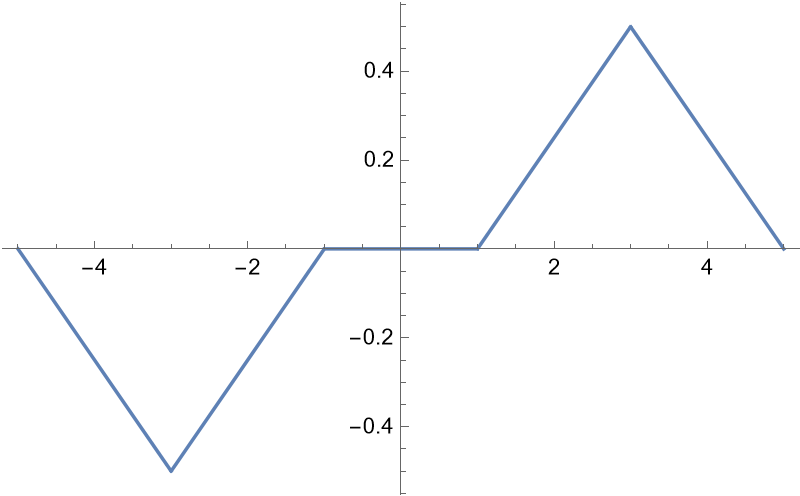
\includegraphics[width=\textwidth]{plots/config-1.5.png}
        \subcaption{$t=1.5$}
    \end{subfigure}
    \begin{subfigure}{0.4\textwidth}
        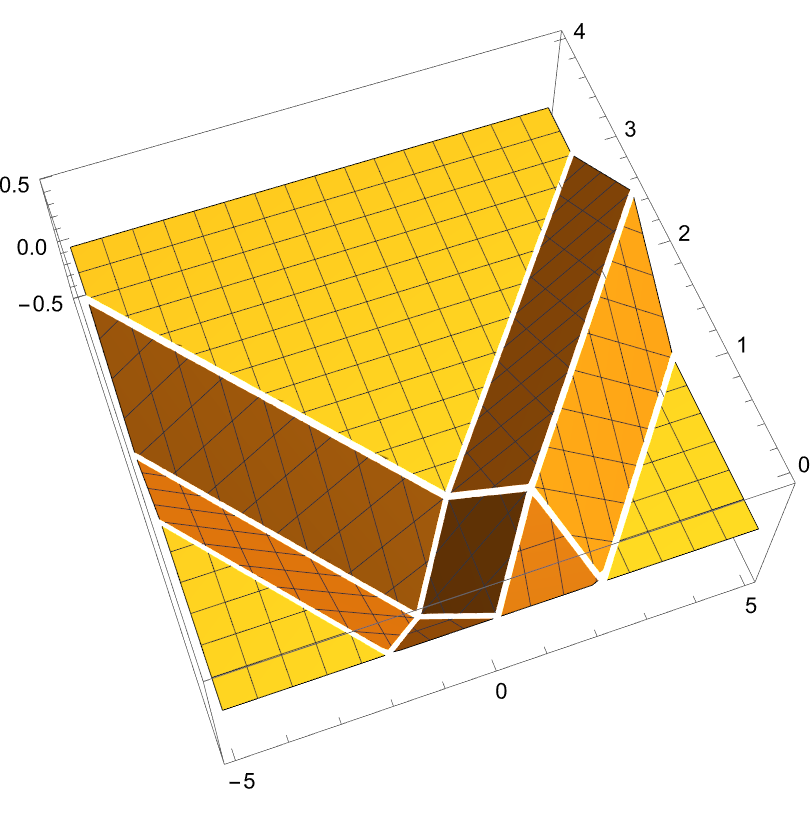
\includegraphics[width=\textwidth]{plots/config-3d.png}
        \subcaption{3D plot; the $y$ axis represents the $t$ variable}
    \end{subfigure}
    \caption{Plot of $y(x, t)$ with different $t$}
    \label{fig:plot-y}
\end{figure}

\section{}

We repeat the procedure in last section, but now with 
\begin{equation}
    \begin{gathered}
        c=4, \\
        f(x)=x^2-2 x \\
        g(x)=\cos x
        \end{gathered}
\end{equation}
Now 
\begin{equation}
    \begin{aligned}
        y(x, t) &= \frac{1}{2} ((x - 4t)^2 - 2 (x - 4t)) + \frac{1}{2} ((x + 4t)^2 - 2 (x + 4t))
        + \frac{1}{8} (\sin (x + 4 t) - \sin(x - 4t)) \\
        &= \underbrace{\frac{1}{2} ((x - 4t)^2 - 2 (x - 4t)) - \frac{1}{8} \sin(x - 4 t)}_{F(x - 4t)}
        + \underbrace{\frac{1}{2} ((x + 4t)^2 - 2 (x + 4t)) + \frac{1}{8} \sin(x + 4 t)}_{G(x + 4t)}.
    \end{aligned}
\end{equation}

The plots of $F$ and $G$ are shown in \prettyref{fig:plot-1}.
It can be seen that the behavior of the solution is dominated by the $x^2 - 2x$ term.
As time goes by, 
the parts of $F$ and $G$ with large $\abs{x}$ moves to the vicinity of $x = 0$,
making $y(x, t)$ larger and larger.
Ignoring the contribution of $g(x)$, we get 
\begin{equation}
    y(x, t) = \frac{1}{2} ((x - 4t)^2 - 2 (x - 4t)) + \frac{1}{2} ((x + 4t)^2 - 2 (x + 4t))
    = x^2 - 2 x + 4 t^2,
\end{equation}
so $y(x, t)$ is roughly a parabolic being moved upwards.

\begin{figure}
    \centering
    \begin{subfigure}{0.45\textwidth}
        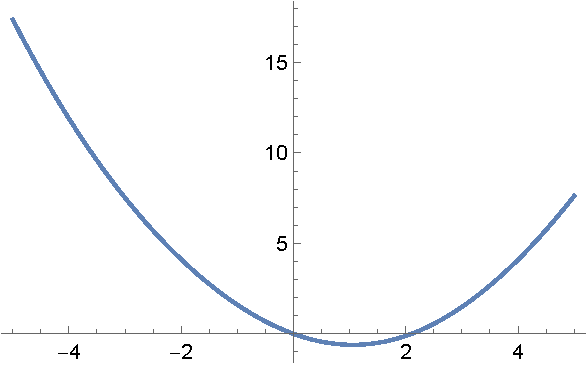
\includegraphics[width=\textwidth]{plots/wave-f-1.pdf}
        \subcaption{}
    \end{subfigure}
    \begin{subfigure}{0.45\textwidth}
        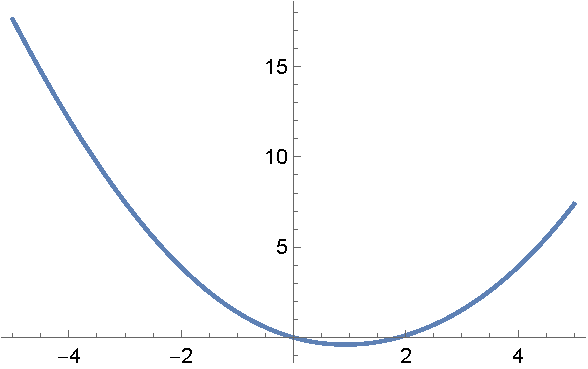
\includegraphics[width=\textwidth]{plots/wave-g-1.pdf}
        \subcaption{}
    \end{subfigure}
    \caption{(a) $F(x)$ (b) $G(x)$}
    \label{fig:plot-1} 
\end{figure}

\section{}

The general solution of $\laplacian u = 0$ in a circle 
(with the implicit boundary condition that $u(r=0)$ should be well-defined)
in polar coordinates, is 
\begin{equation}
    u(r, \theta)=a_0+\sum_{n=1}^{\infty}\left[a_n r^n \cos (n \theta)+b_n r^n \sin (n \theta)\right].
\end{equation}
The boundary condition 
\begin{equation}
    u(r = 5, \theta) = \theta \cos \theta
\end{equation}
then means 
\begin{equation}
    2\pi a_0 = \int_{0}^{2\pi} \theta \cos \theta \dd{\theta} = 0,
\end{equation}
\begin{equation}
    \pi \cdot a_n \cdot 5^n = \int_{0}^{2\pi} \cos(n \theta) \cdot \theta \cos \theta \dd{\theta} = 0,
\end{equation}
and 
\begin{equation}
    \pi \cdot b_n \cdot 5^n = \int_{0}^{2\pi} \sin(n \theta) \cdot \theta \cos \theta \dd{\theta} 
    = \begin{cases}
        - \frac{\pi}{2}, &n = 2, \\
        - \frac{2n \pi}{n^2 - 1}, & \text{otherwise}.
    \end{cases}
\end{equation}
So we have 
\begin{equation}
    u(r, \theta) = - \frac{1}{10} r \sin \theta - \sum_{n=2}^{\infty} \frac{r^n}{5^n} \frac{2n}{n^2 - 1} \sin n \theta.
\end{equation}

\end{document}